\documentclass[final]{beamer} % beamer 3.10: do NOT use option hyperref={pdfpagelabels=false} !
\mode<presentation> {  %% check http://www-i6.informatik.rwth-aachen.de/~dreuw/latexbeamerposter.php for examples
  \usetheme{Berlin}    %% you should define your own theme e.g. for big headlines using your own logos
}
%height=121.92
%\usepackage[english]{babel}
\usepackage{amsmath,amsthm, amssymb, latexsym}
\usepackage[size=custom,width=182.88,height=128.92,scale=2]{beamerposter}
\usepackage{array}
\usepackage{wrapfig}

\setlength{\voffset}{1in}
\setlength{\topmargin}{0in}
\setlength{\footskip}{0in}
\setlength{\headheight}{0in}
\setlength{\headsep}{0in}


\setlength{\hoffset}{0in}
\setlength{\oddsidemargin}{1.5in}
\setlength{\textwidth}{67.5in}
\parindent 0in

%\setlength{\oddsidemargin}{2.5in}
%\setlength{\topmargin}{2.5in}
%\setlength{\textwidth}{67in}
%\setlength{\textheight}{43in}

% e.g. for custom size poster
\title{Generating Safe Trajectories in Stochastic Dynamic Environments by
    Leveraging Information about Obstacle Motion}
    \author{Alex Wallar | \emph{Supervisor}: Michael Weir}
\institute{School of Computer Science, University of St Andrews}
%\date{Jul. 27th, 2011}

%\input{pstyle}


\newcommand{\Acronym}[1]{\ensuremath{{{\texttt{#1}}}}}
\newcommand{\Symbol}[1]{\ensuremath{\mathcal{#1}}}
\newcommand{\Function}[1]{\ensuremath{{\textsc{#1}}}}
\newcommand{\Constant}[1]{\ensuremath{{\texttt{#1}}}}
\newcommand{\Var}[1]{\ensuremath{{{\mathrm{#1}}}}}
\newcommand{\False}{\Constant{false}}
\newcommand{\True}{\Constant{true}}
\newcommand{\Null}{\Constant{null}}
\newcommand{\R}{\ensuremath{\mathbb{R}}}
\newcommand{\AlgoFont}[1]{\footnotesize{#1}}
\newcommand{\RefFont}[1]{\tiny{#1}}


\definecolor{boxrgb}{rgb}{0.7,0.9,0.7}
\setbeamercolor{mybox1}{fg=black,bg=boxrgb}
\setbeamercolor{mybox2}{fg=red,bg=boxrgb}

\definecolor{mathrgb}{rgb}{0.0,0.0,0.74}

\definecolor{proBlockTitleFG}{rgb}{0.95,0.95,0.00}
\definecolor{proBlockTitleBG}{rgb}{0.21,0.26,0.42}
\definecolor{proBlockBodyBG}{rgb}{0.94,0.94,0.97}


\definecolor{hTitleFG}{rgb}{0.95,0.95,0.00}
\definecolor{hAuthorFG}{rgb}{1, 1, 1}
\definecolor{hInstFG}{rgb}{1, 1, 1}
\definecolor{hInfoFG}{rgb}{1, 1, 1}
\definecolor{hBG}{rgb}{0.11,0.16,0.32}

\definecolor{mytitle_bg}{rgb}{0.4,0.4,0.4}
\newcommand{\myimp}[1]{{\textcolor{mytitle_bg}{\textbf{#1}}}}
\newcommand{\myhimp}[1]{{\textcolor{red}{\textbf{#1}}}}
\newcommand{\mymath}[1]{\textcolor{mathrgb}{#1}}

\graphicspath{{../}}

\setbeamercolor{headline}{fg=red,bg=hBG}

\setbeamertemplate{headline}{
  \leavevmode

        \begin{beamercolorbox}[wd=67.5in,ht=5.8in]{headline}


\centering
%\hspace*{3.2in}
\begin{tabular}{c}
\\[-7cm]
         \textcolor{hTitleFG}{\textbf{\huge{Dodger: Generating Safe Trajectories
               in Stochastic Dynamic Environments}}}\\[2cm]
         \textcolor{hTitleFG}{\textbf{\huge{ by Leveraging Information about Obstacle Motion}}}\\[3cm]


        \textcolor{hAuthorFG}{\textbf{\huge{\insertauthor}}}\\[1.8cm]

        \textcolor{hInstFG}{\Large{\insertinstitute}}\\[1.5cm]


       % \textcolor{hInfoFG}{{\large{http://faculty.cua.edu/plaku,
        %      \texttt{plaku@cua.edu}}}}\\[0.5cm]
\end{tabular}

        \end{beamercolorbox}

  \begin{beamercolorbox}[wd=\paperwidth]{lower separation line head}
    \rule{0pt}{3pt}
  \end{beamercolorbox}
}
\setbeamertemplate{footline}{}

\setbeamertemplate{navigation symbols}{}


\newenvironment<>{problock}[1]{%
  \begin{actionenv}#2%
      \def\insertblocktitle{
\begin{beamercolorbox}[ht=1in,center]{proBlockTitleBG}
 \vbox to 1in{\vfil \centering {\Large \textbf{#1}} \vfil}%
\end{beamercolorbox}
}

      \par%
       \setbeamerfont{block body}{size=\normalsize}
       \setbeamercolor{block title}{fg=proBlockTitleFG,bg=proBlockTitleBG}
       \setbeamercolor{block body}{fg=black,bg=white}%,bg=proBlockBodyBG}
       \setbeamercolor{itemize item}{fg=orange!20!black}
       \setbeamertemplate{itemize item}[circle]
      \usebeamertemplate{block begin}\vspace*{1cm}}
    {\par\usebeamertemplate{block end}\end{actionenv}}

\begin{document}

\vspace*{-50mm}

  \begin{frame}{}
\noindent
    \begin{columns}[t]
      \begin{column}{21.6in}
        \begin{problock}{1. PROBLEM FORMULATION}

\begin{itemize}
    \item Develop a probabilistic representation of dynamic obstacles that
        accounts for their motion
    \item Use this representation to build a cost distribution that can
        be used as a heuristic to guide the search
    \item Generate a trajectory for a robot that reaches the goal region
        whilst avoiding collisions with static and dynamic obstacles
    \item Utilize information about the motion of obstacles and their
        associated cost distributions
    \item Replan if the obstacles deviate a significant amount from their
        predicted paths
\end{itemize}


        \end{problock}

\begin{problock}{3. EXPERIMENTAL RESULTS}

The figure below shows the average minimum distance to any obstacle compared
to a potential fields planner as the speed increases. The higher the minimum
distance to an obstacle, the safer the path.
\vspace*{8mm}

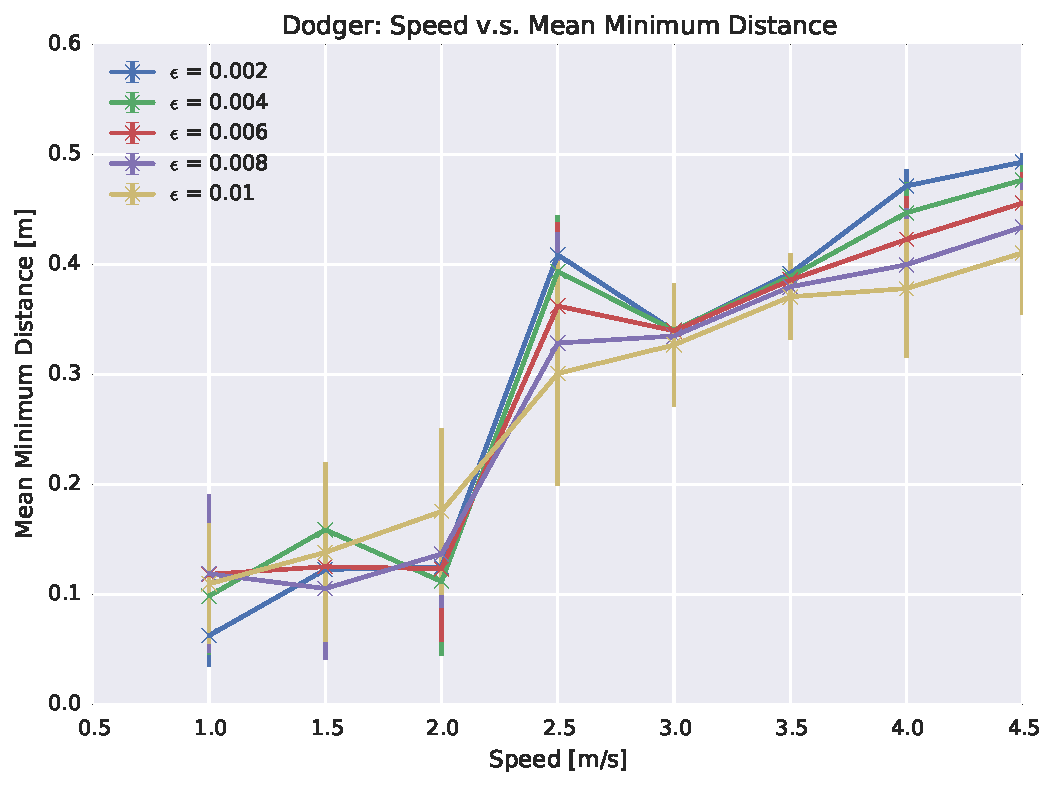
\includegraphics[width=0.49\textwidth]{figs/planner_mean_min_distance_0.pdf}
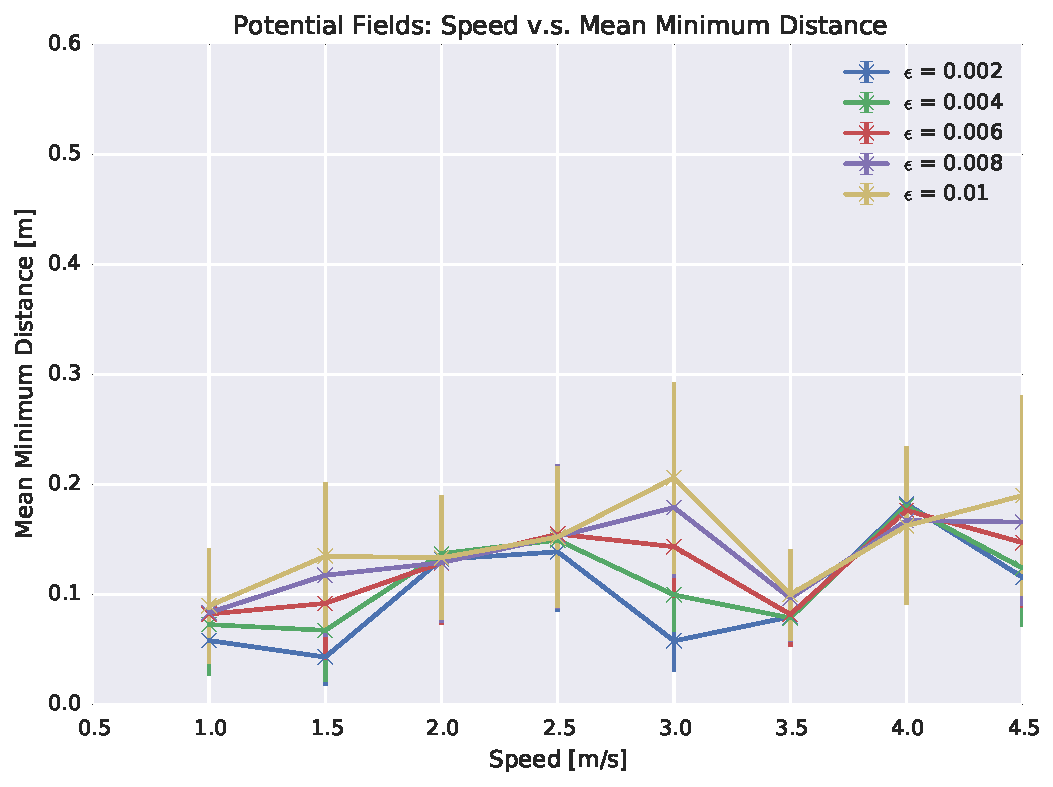
\includegraphics[width=0.49\textwidth]{figs/pf_mean_min_distance_0.pdf}

% \begin{itemize}
%     \item Each line shows a different amount of noise injected into the
%         obstacle trajectories
% \end{itemize}

\vspace*{10mm}

The figure below shows the maximum cost incurred by the robot along the paths generated by Dodger and
a potential fields planner. The cost is defined by the cost distribution
given by the dynamic obstacle representation. The lower the cost, the safer
the path.

\vspace*{10mm}
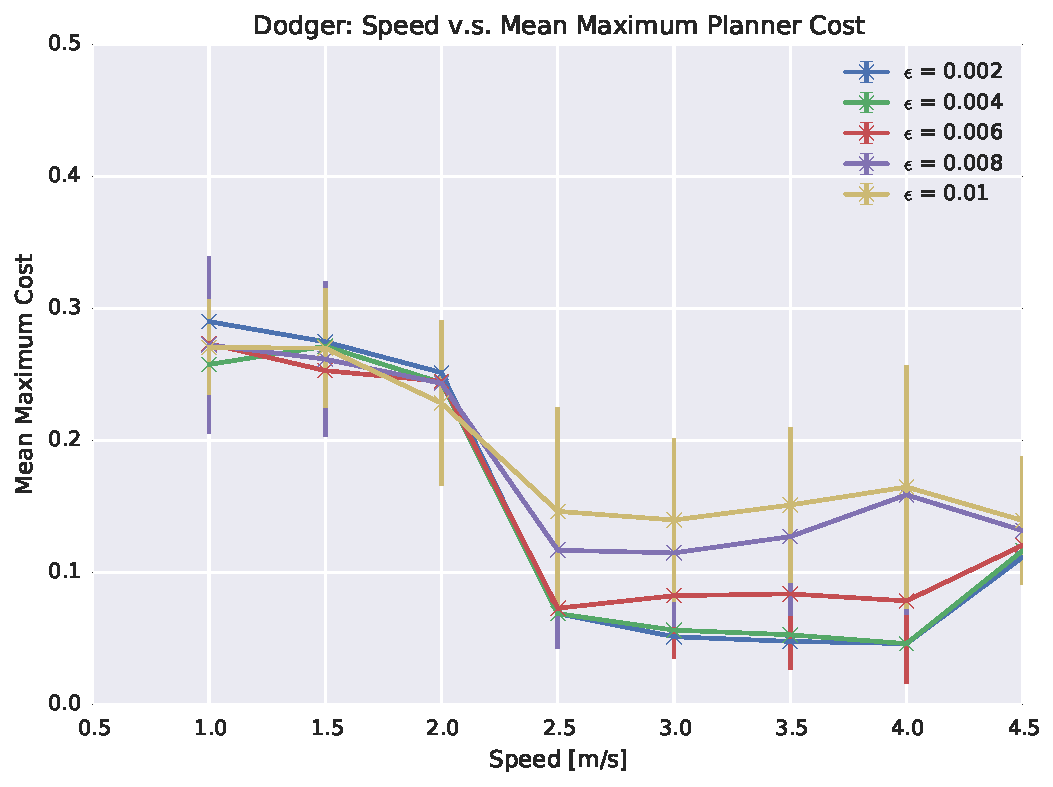
\includegraphics[width=0.49\textwidth]{figs/planner_mean_max_cost_0.pdf}
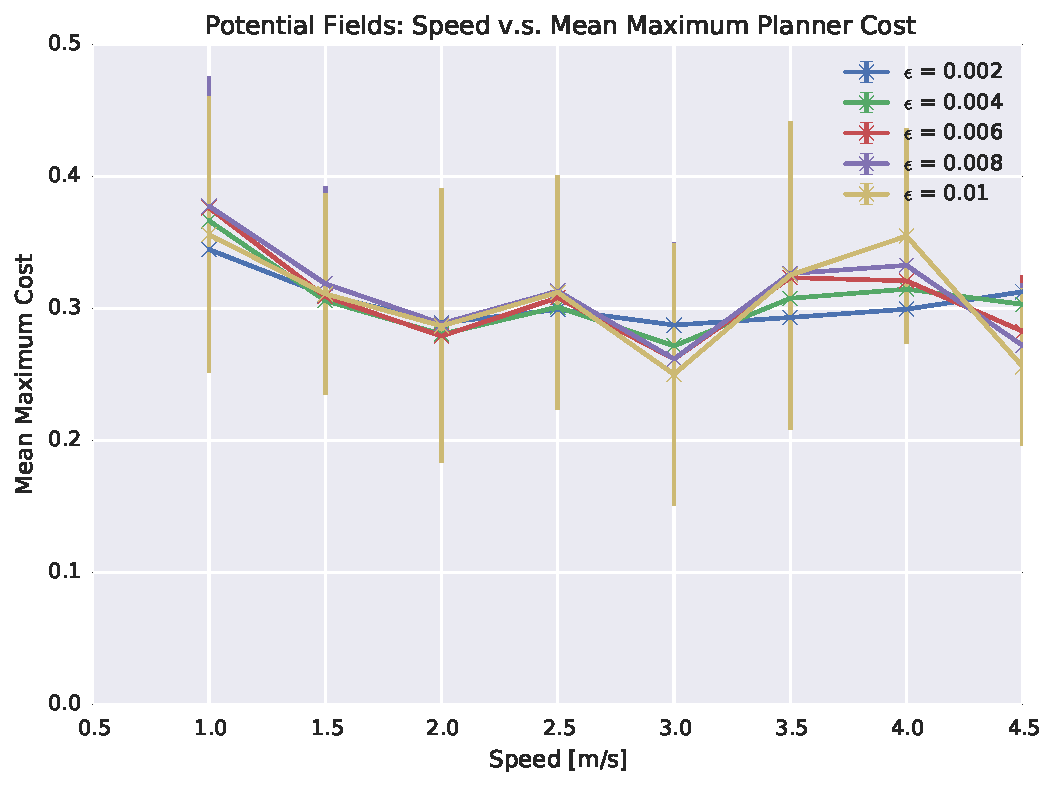
\includegraphics[width=0.49\textwidth]{figs/pf_mean_max_cost_0.pdf}\\
\vspace*{30mm}

\includegraphics[width=0.10\linewidth]{figs/st-andrews-logo}
\hspace*{3mm}

\includegraphics[width=0.5\linewidth]{figs/sicsa}
\end{problock}

      \end{column}

%%%%%%%%%%%%%%%%%%%%%%%%%%%%%%%%%%%%%%%
      \begin{column}{43in}
        \begin{problock}{2. APPROACH}

% {\centerline{
% 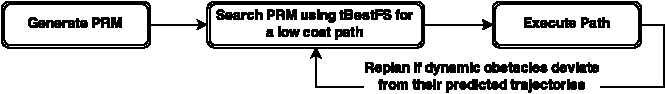
\includegraphics[width=1\columnwidth]{figs/DodgerScheme}
% }}

\begin{columns}[t]

\column{0.48\columnwidth}

\textcolor{red}{\textbf{\large{1. Dynamic Obstacle Representation}}}

\vspace*{8mm}

% A dynamic obstacle is represented by five variables:
% \begin{itemize}
%     \item $I$ is the initial configuration of the obstacle,
%     \item $\dot{\zeta}$ is a function, $\dot{\zeta}: \mathbb{R}^+ \rightarrow
% \mathbb{R}^2$, representing the velocity of the obstacle
%     \item $\epsilon$ is used to define a random variable
%         $\rho \sim \mathcal{U}(-\epsilon, \epsilon)$
%     \item $\xi$ is the last known configuration of the obstacle used for
%         extrapolation
%     \item $T$ is the time at which $\xi$ was recorded
% \end{itemize}
% 
% The cost distribution for a single dynamic obstacle used as a heuristic
% for planning is:
% \begin{equation*}
%     P_a(x, y, t_0, t_m) = \frac{1}{t_m} \cdot \int^{t_m}_{t_0}
%     \mathcal{N}(\zeta_a(t), \alpha \cdot (t - t_0)^2 + \beta, x, y) \cdot
%     (t_m - t + 1)^{\gamma} \,\mathrm{d}t
%     \label{eq:singleprob}
% \end{equation*}
% 
% Where $[t_0, t_m]$ defines the interval for which the cost distribution is
% evaluated on. This serves to represent the likelihood of an obstacle moving
% to an $(x, y)$ location between for a time $t$ such that $t_0 \leq t \leq t_m$

A stochastic representation has been developed that accounts for the
trajectories of dynamic obstacles. The figure below represents the cost incurred
by a robot moving to a certain location in the environment for a given
time period. This scene has two obstacles moving side to side in a sinusoidal fashion.

\vspace*{8mm}

\begin{center}
    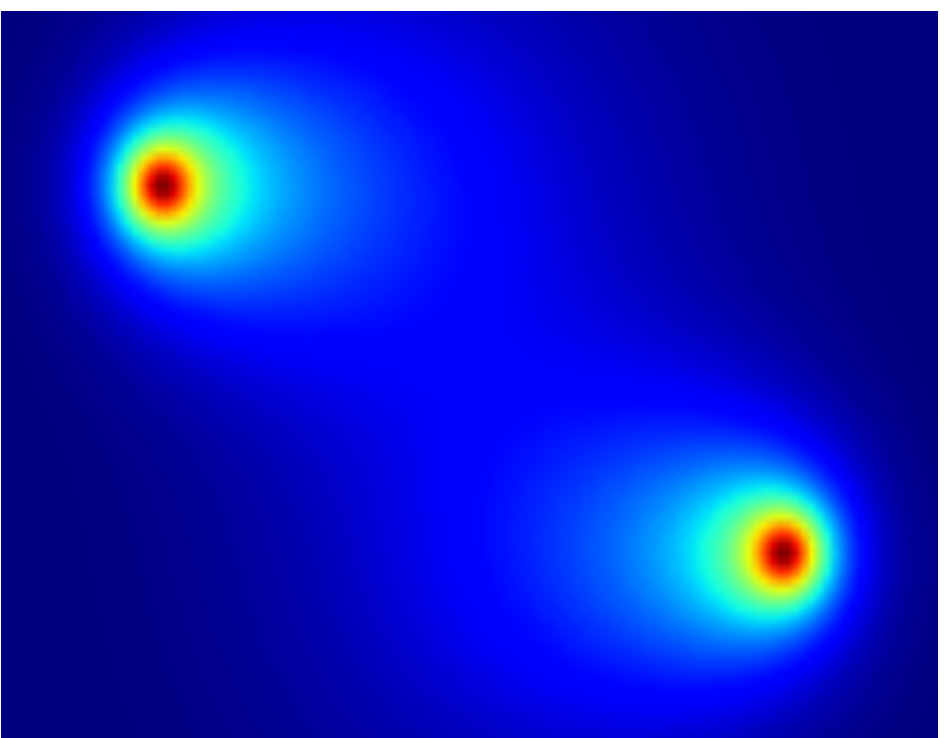
\includegraphics[width=0.4\linewidth]{figs/agent_1-crop}
    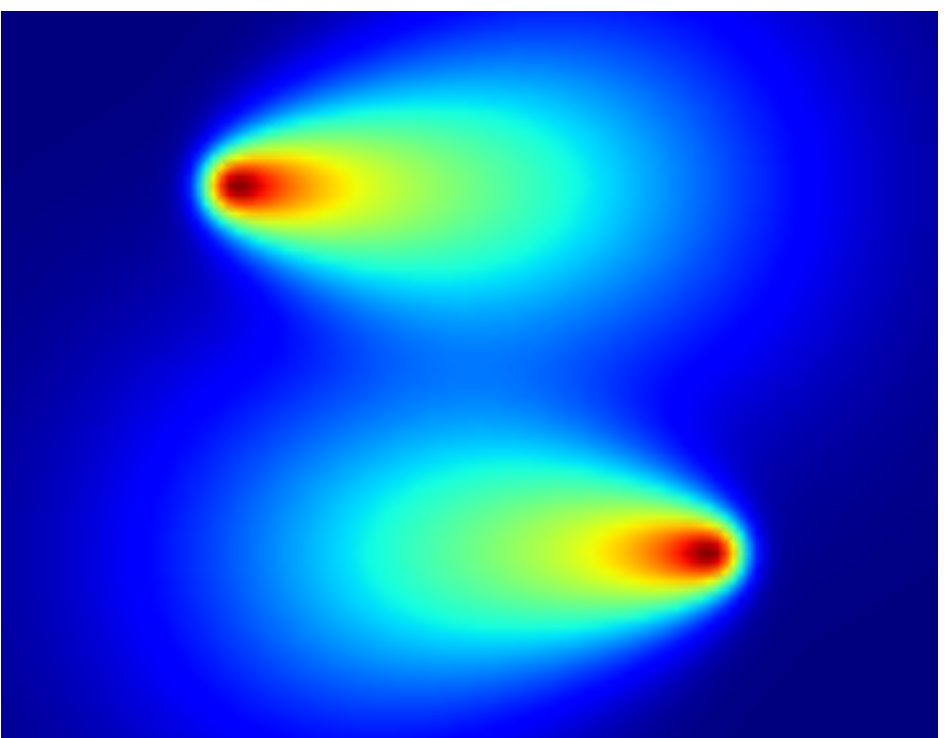
\includegraphics[width=0.4\linewidth]{figs/agent_3-crop} \\
    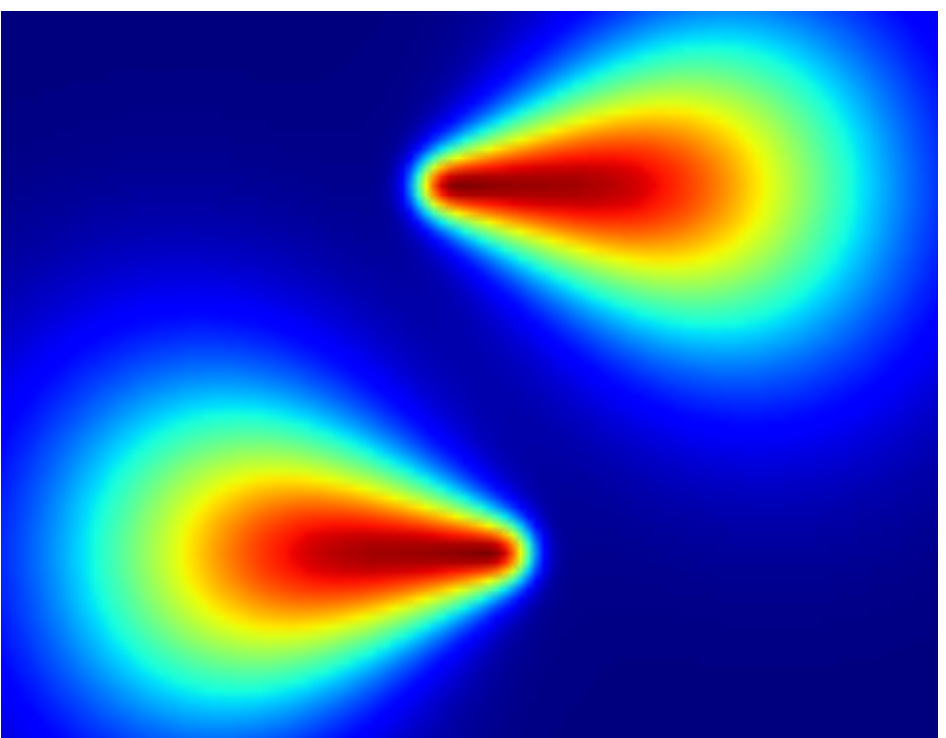
\includegraphics[width=0.4\linewidth]{figs/agent_5-crop}
    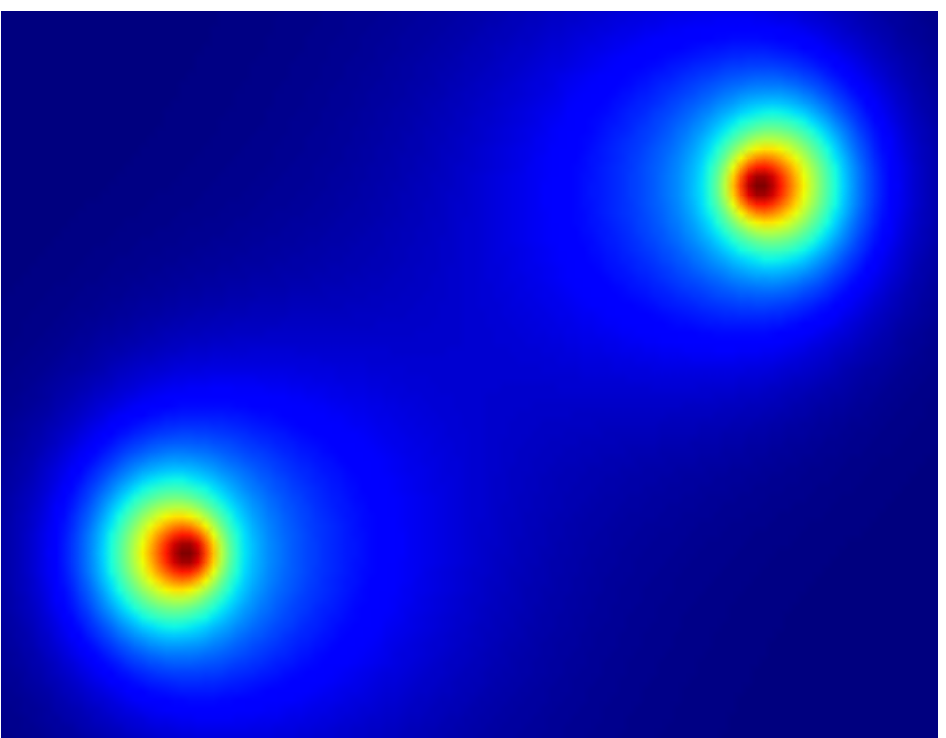
\includegraphics[width=0.4\linewidth]{figs/agent_8-crop}
\end{center}

\vspace*{8mm}

\textcolor{red}{\textbf{\large{2. Generating the Probabilistic Roadmap (PRM)}}}

\vspace*{8mm}

A PRM is a graph that is generated by randomly sampling points in the environment
and adding an edge between two points if their within some distance. It is
constructed over the configuration space of the robot and is used to guide the
expansion of the temporal graph search. An example PRM is shown below.

\begin{center}
    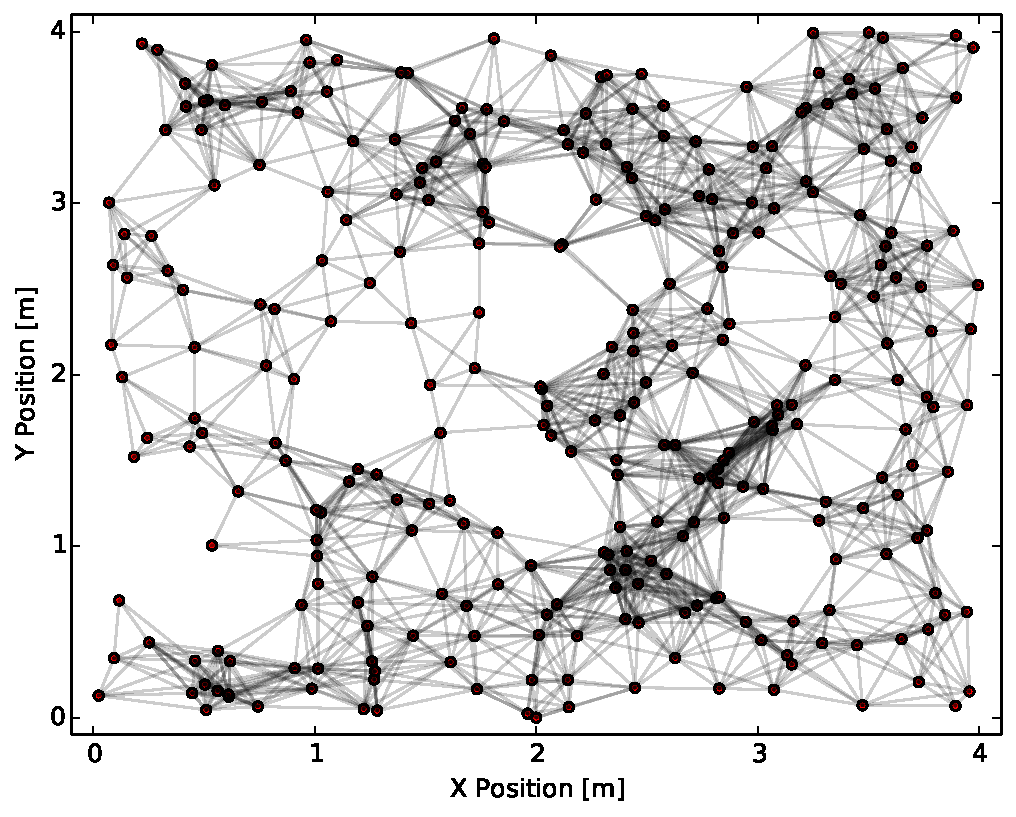
\includegraphics[width=0.7\textwidth]{figs/roadmap}
\end{center}

\column{0.48\columnwidth}

\textcolor{red}{\textbf{\large{3. Searching the PRM}}}

\vspace*{8mm}

A novel search algorithm has been developed to search the probabilistic
roadmap to find low cost paths where the cost is dynamic and time-dependent.

\begin{center}
    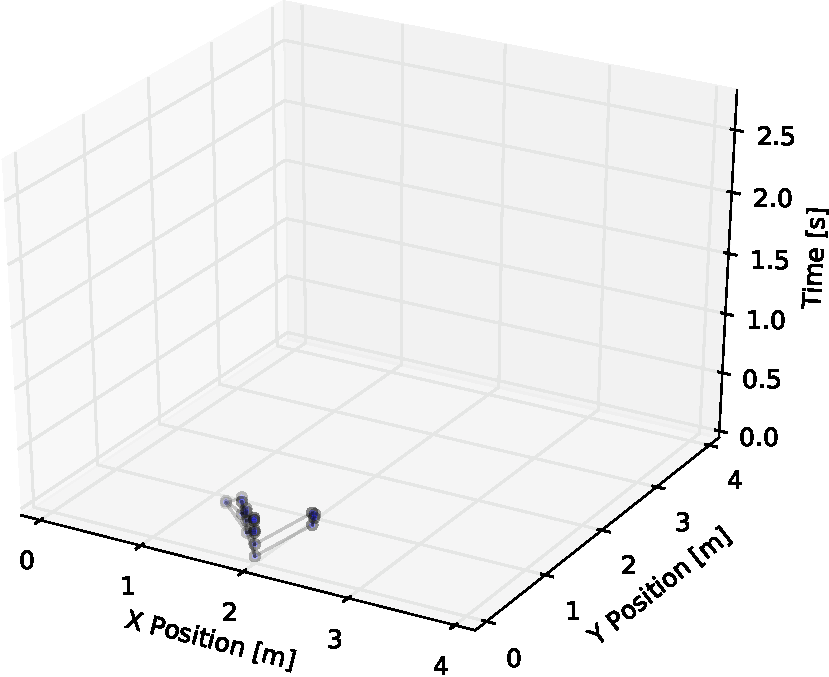
\includegraphics[width=0.35\linewidth]{figs/tree_1-crop}
    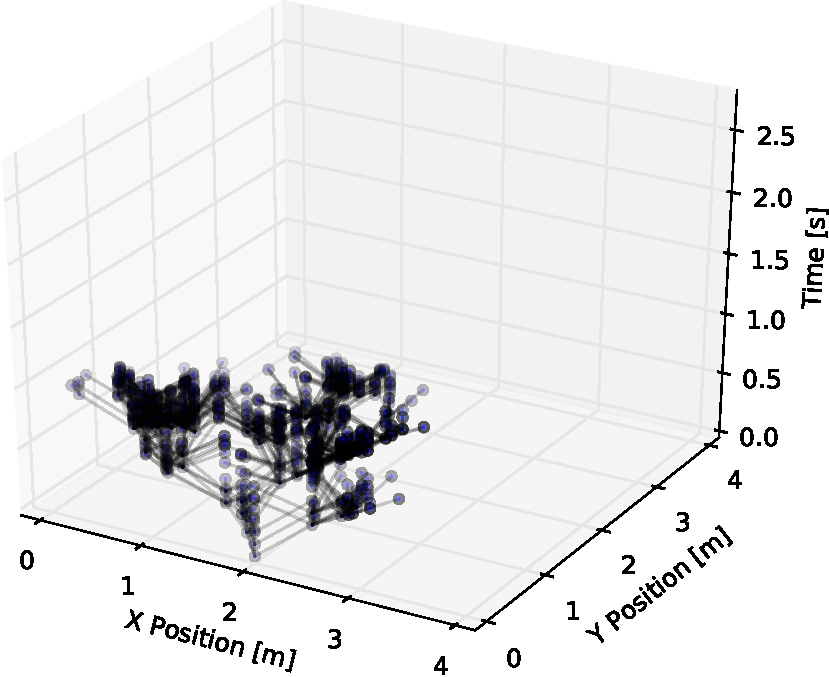
\includegraphics[width=0.35\linewidth]{figs/tree_3-crop} \\
    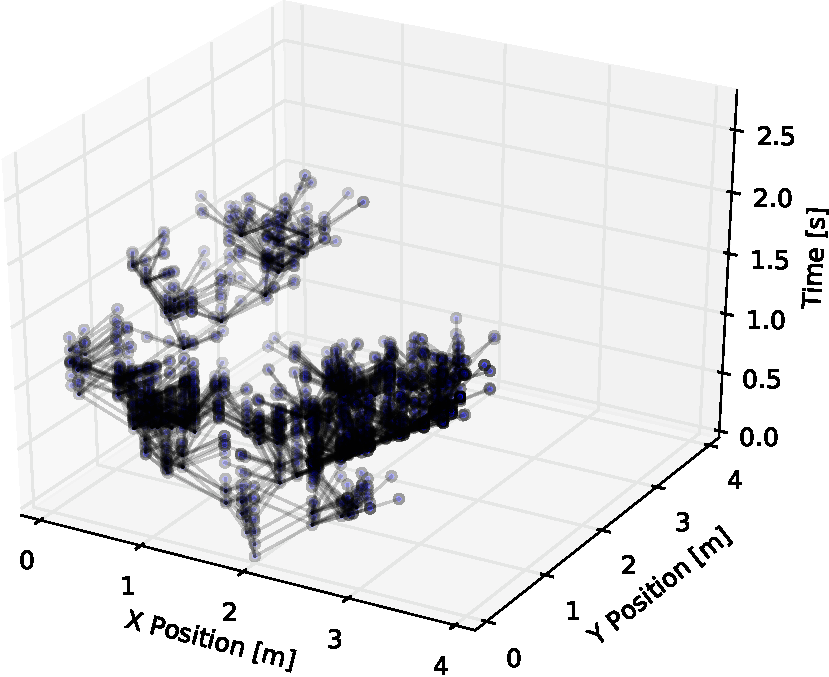
\includegraphics[width=0.35\linewidth]{figs/tree_6-crop}
    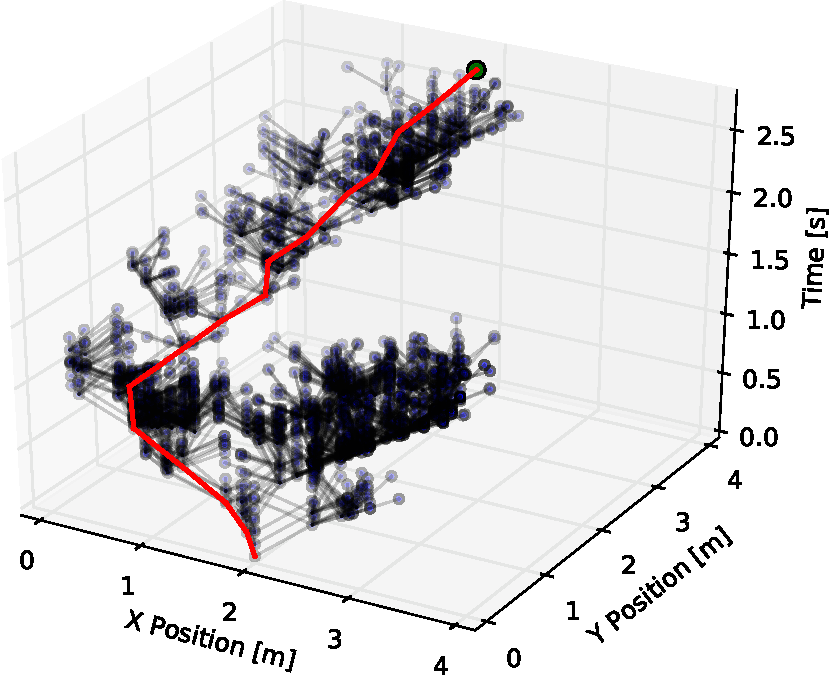
\includegraphics[width=0.35\linewidth]{figs/tree_8-crop}
\end{center}

\vspace*{10mm}

\textcolor{red}{\textbf{\large{4. Replanning}}}

\vspace*{8mm}

Information about obstacle motion is not perfect and the plan may need to
adapt to changes in the predicted environment.

\begin{center}
    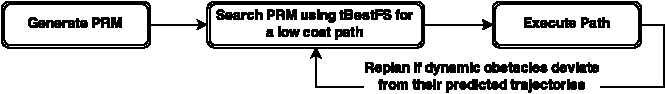
\includegraphics[width=1\columnwidth]{figs/DodgerScheme}
\end{center}

Below is a figure showing the progression of the path around stochastic
dynamic obstacles.

\begin{center}
    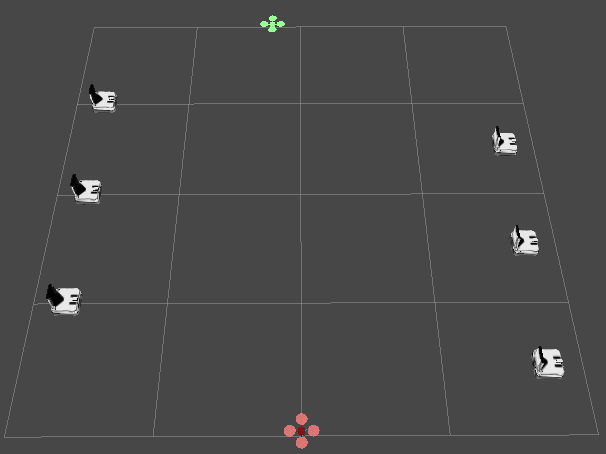
\includegraphics[width=0.4\linewidth]{figs/dodger_0-crop}
    \hspace*{2mm}
    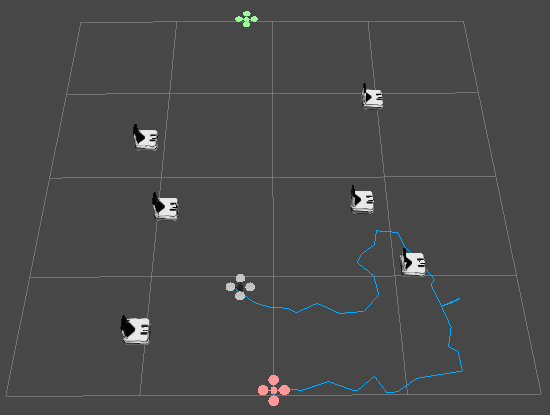
\includegraphics[width=0.4\linewidth]{figs/dodger_8-crop} \\
    \vspace*{2mm}
    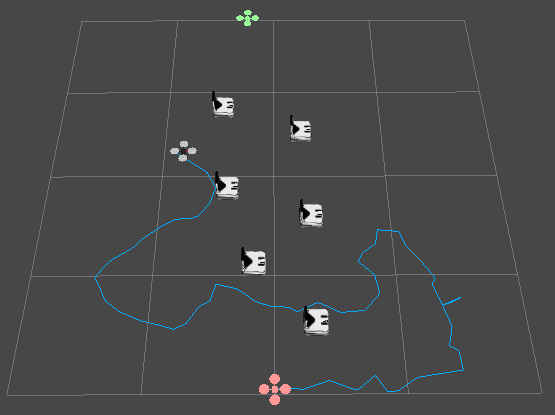
\includegraphics[width=0.4\linewidth]{figs/dodger_13-crop}
    \hspace*{2mm}
    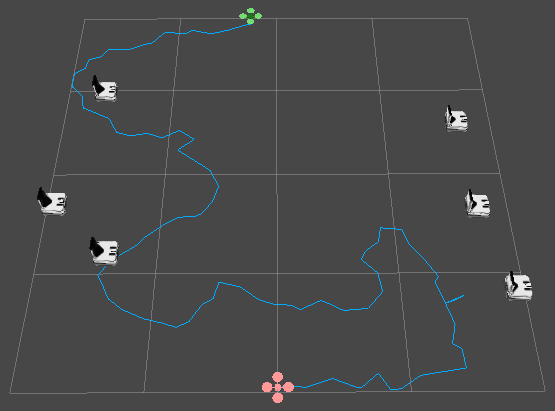
\includegraphics[width=0.4\linewidth]{figs/dodger_complete}
\end{center}
\end{columns}
\end{problock}
\end{column}
\end{columns}
\end{frame}
\end{document}
